% Options for packages loaded elsewhere
\PassOptionsToPackage{unicode}{hyperref}
\PassOptionsToPackage{hyphens}{url}
%
\documentclass[
]{article}
\author{}
\date{\vspace{-2.5em}}

\usepackage{amsmath,amssymb}
\usepackage{lmodern}
\usepackage{iftex}
\ifPDFTeX
  \usepackage[T1]{fontenc}
  \usepackage[utf8]{inputenc}
  \usepackage{textcomp} % provide euro and other symbols
\else % if luatex or xetex
  \usepackage{unicode-math}
  \defaultfontfeatures{Scale=MatchLowercase}
  \defaultfontfeatures[\rmfamily]{Ligatures=TeX,Scale=1}
\fi
% Use upquote if available, for straight quotes in verbatim environments
\IfFileExists{upquote.sty}{\usepackage{upquote}}{}
\IfFileExists{microtype.sty}{% use microtype if available
  \usepackage[]{microtype}
  \UseMicrotypeSet[protrusion]{basicmath} % disable protrusion for tt fonts
}{}
\makeatletter
\@ifundefined{KOMAClassName}{% if non-KOMA class
  \IfFileExists{parskip.sty}{%
    \usepackage{parskip}
  }{% else
    \setlength{\parindent}{0pt}
    \setlength{\parskip}{6pt plus 2pt minus 1pt}}
}{% if KOMA class
  \KOMAoptions{parskip=half}}
\makeatother
\usepackage{xcolor}
\IfFileExists{xurl.sty}{\usepackage{xurl}}{} % add URL line breaks if available
\IfFileExists{bookmark.sty}{\usepackage{bookmark}}{\usepackage{hyperref}}
\hypersetup{
  hidelinks,
  pdfcreator={LaTeX via pandoc}}
\urlstyle{same} % disable monospaced font for URLs
\usepackage[margin=1in]{geometry}
\usepackage{color}
\usepackage{fancyvrb}
\newcommand{\VerbBar}{|}
\newcommand{\VERB}{\Verb[commandchars=\\\{\}]}
\DefineVerbatimEnvironment{Highlighting}{Verbatim}{commandchars=\\\{\}}
% Add ',fontsize=\small' for more characters per line
\usepackage{framed}
\definecolor{shadecolor}{RGB}{248,248,248}
\newenvironment{Shaded}{\begin{snugshade}}{\end{snugshade}}
\newcommand{\AlertTok}[1]{\textcolor[rgb]{0.94,0.16,0.16}{#1}}
\newcommand{\AnnotationTok}[1]{\textcolor[rgb]{0.56,0.35,0.01}{\textbf{\textit{#1}}}}
\newcommand{\AttributeTok}[1]{\textcolor[rgb]{0.77,0.63,0.00}{#1}}
\newcommand{\BaseNTok}[1]{\textcolor[rgb]{0.00,0.00,0.81}{#1}}
\newcommand{\BuiltInTok}[1]{#1}
\newcommand{\CharTok}[1]{\textcolor[rgb]{0.31,0.60,0.02}{#1}}
\newcommand{\CommentTok}[1]{\textcolor[rgb]{0.56,0.35,0.01}{\textit{#1}}}
\newcommand{\CommentVarTok}[1]{\textcolor[rgb]{0.56,0.35,0.01}{\textbf{\textit{#1}}}}
\newcommand{\ConstantTok}[1]{\textcolor[rgb]{0.00,0.00,0.00}{#1}}
\newcommand{\ControlFlowTok}[1]{\textcolor[rgb]{0.13,0.29,0.53}{\textbf{#1}}}
\newcommand{\DataTypeTok}[1]{\textcolor[rgb]{0.13,0.29,0.53}{#1}}
\newcommand{\DecValTok}[1]{\textcolor[rgb]{0.00,0.00,0.81}{#1}}
\newcommand{\DocumentationTok}[1]{\textcolor[rgb]{0.56,0.35,0.01}{\textbf{\textit{#1}}}}
\newcommand{\ErrorTok}[1]{\textcolor[rgb]{0.64,0.00,0.00}{\textbf{#1}}}
\newcommand{\ExtensionTok}[1]{#1}
\newcommand{\FloatTok}[1]{\textcolor[rgb]{0.00,0.00,0.81}{#1}}
\newcommand{\FunctionTok}[1]{\textcolor[rgb]{0.00,0.00,0.00}{#1}}
\newcommand{\ImportTok}[1]{#1}
\newcommand{\InformationTok}[1]{\textcolor[rgb]{0.56,0.35,0.01}{\textbf{\textit{#1}}}}
\newcommand{\KeywordTok}[1]{\textcolor[rgb]{0.13,0.29,0.53}{\textbf{#1}}}
\newcommand{\NormalTok}[1]{#1}
\newcommand{\OperatorTok}[1]{\textcolor[rgb]{0.81,0.36,0.00}{\textbf{#1}}}
\newcommand{\OtherTok}[1]{\textcolor[rgb]{0.56,0.35,0.01}{#1}}
\newcommand{\PreprocessorTok}[1]{\textcolor[rgb]{0.56,0.35,0.01}{\textit{#1}}}
\newcommand{\RegionMarkerTok}[1]{#1}
\newcommand{\SpecialCharTok}[1]{\textcolor[rgb]{0.00,0.00,0.00}{#1}}
\newcommand{\SpecialStringTok}[1]{\textcolor[rgb]{0.31,0.60,0.02}{#1}}
\newcommand{\StringTok}[1]{\textcolor[rgb]{0.31,0.60,0.02}{#1}}
\newcommand{\VariableTok}[1]{\textcolor[rgb]{0.00,0.00,0.00}{#1}}
\newcommand{\VerbatimStringTok}[1]{\textcolor[rgb]{0.31,0.60,0.02}{#1}}
\newcommand{\WarningTok}[1]{\textcolor[rgb]{0.56,0.35,0.01}{\textbf{\textit{#1}}}}
\usepackage{graphicx}
\makeatletter
\def\maxwidth{\ifdim\Gin@nat@width>\linewidth\linewidth\else\Gin@nat@width\fi}
\def\maxheight{\ifdim\Gin@nat@height>\textheight\textheight\else\Gin@nat@height\fi}
\makeatother
% Scale images if necessary, so that they will not overflow the page
% margins by default, and it is still possible to overwrite the defaults
% using explicit options in \includegraphics[width, height, ...]{}
\setkeys{Gin}{width=\maxwidth,height=\maxheight,keepaspectratio}
% Set default figure placement to htbp
\makeatletter
\def\fps@figure{htbp}
\makeatother
\setlength{\emergencystretch}{3em} % prevent overfull lines
\providecommand{\tightlist}{%
  \setlength{\itemsep}{0pt}\setlength{\parskip}{0pt}}
\setcounter{secnumdepth}{-\maxdimen} % remove section numbering
\usepackage{booktabs}
\usepackage{longtable}
\usepackage{array}
\usepackage{multirow}
\usepackage{wrapfig}
\usepackage{float}
\usepackage{colortbl}
\usepackage{pdflscape}
\usepackage{tabu}
\usepackage{threeparttable}
\usepackage{threeparttablex}
\usepackage[normalem]{ulem}
\usepackage{makecell}
\usepackage{xcolor}
\ifLuaTeX
  \usepackage{selnolig}  % disable illegal ligatures
\fi

\begin{document}

\hypertarget{intro-to-r-day-3}{%
\section{Intro to R Day 3}\label{intro-to-r-day-3}}

\begin{center}\rule{0.5\linewidth}{0.5pt}\end{center}

Load your day 2 workspace data:

\begin{Shaded}
\begin{Highlighting}[]
\FunctionTok{load}\NormalTok{(}\StringTok{"day2.RData"}\NormalTok{)}
\end{Highlighting}
\end{Shaded}

\hypertarget{loops}{%
\subsubsection{Loops}\label{loops}}

In programming, it is common that one has to do one set of specific
operation on a sequence of elements. In this case, \emph{for} loop is
very useful to achieve the goal.

The basic structure of \emph{for} loop is:

\textbf{for (value in sequence)\{}

\textbf{some operation}

\textbf{\}}

For example, we would like to calculate the sum of a row for every row
in the matrix we created earlier. We are going to use a \emph{for} loop
to do it.

\begin{Shaded}
\begin{Highlighting}[]
\ControlFlowTok{for}\NormalTok{ (i }\ControlFlowTok{in} \DecValTok{1}\SpecialCharTok{:}\FunctionTok{dim}\NormalTok{(my\_matrix)[}\DecValTok{1}\NormalTok{]) \{}
\NormalTok{  out }\OtherTok{\textless{}{-}} \FunctionTok{sum}\NormalTok{(my\_matrix[i, ])}
  \FunctionTok{print}\NormalTok{(out)}
\NormalTok{\}}
\end{Highlighting}
\end{Shaded}

\begin{verbatim}
## [1] 11
## [1] 58
## [1] 302
## [1] 38
\end{verbatim}

There is a \textbf{while} loop in R similarly as in command line or any
other programming language. The basic structure of a \emph{while} loop
is:

\textbf{while (condition)\{}

\textbf{some operation}

\textbf{\}}

Here is the same row sum calculation using a while loop:

\begin{Shaded}
\begin{Highlighting}[]
\ControlFlowTok{while}\NormalTok{ (i }\SpecialCharTok{\textless{}=} \FunctionTok{dim}\NormalTok{(my\_matrix)[}\DecValTok{1}\NormalTok{])\{}
\NormalTok{  out }\OtherTok{\textless{}{-}} \FunctionTok{sum}\NormalTok{(my\_matrix[i,])}
  \FunctionTok{print}\NormalTok{(out)}
\NormalTok{  i }\OtherTok{\textless{}{-}}\NormalTok{ i }\SpecialCharTok{+} \DecValTok{1}
\NormalTok{\}}
\end{Highlighting}
\end{Shaded}

\begin{verbatim}
## [1] 38
\end{verbatim}

\begin{center}\rule{0.5\linewidth}{0.5pt}\end{center}

\hypertarget{the-apply-family-of-functions}{%
\subsubsection{The ``apply'' family of
functions}\label{the-apply-family-of-functions}}

\hypertarget{a-few-useful-functions-apply-lapply-sapply-and-tapply-to-replace-for-loop}{%
\paragraph{A few useful functions: apply(), lapply(), sapply(), and
tapply() to replace for
loop}\label{a-few-useful-functions-apply-lapply-sapply-and-tapply-to-replace-for-loop}}

\hypertarget{apply-takes-an-array-or-matrix-as-input-and-outputs-a-vector-array-or-list.}{%
\subparagraph{apply() takes an array or matrix as input and outputs a
vector, array or
list.}\label{apply-takes-an-array-or-matrix-as-input-and-outputs-a-vector-array-or-list.}}

\begin{Shaded}
\begin{Highlighting}[]
\CommentTok{\# recall my\_matrix}
\NormalTok{my\_matrix}
\end{Highlighting}
\end{Shaded}

\begin{verbatim}
##      col1 col2 col3
## row1    1    2    8
## row2    3   18   37
## row3    8   27  267
## row4    9   10   19
\end{verbatim}

\begin{Shaded}
\begin{Highlighting}[]
\CommentTok{\# check the usage of apply() function}
\NormalTok{?}\FunctionTok{apply}\NormalTok{()}
\CommentTok{\# calculate sums for each row}
\FunctionTok{apply}\NormalTok{(my\_matrix, }\AttributeTok{MARGIN=}\DecValTok{1}\NormalTok{, sum)}
\end{Highlighting}
\end{Shaded}

\begin{verbatim}
## row1 row2 row3 row4 
##   11   58  302   38
\end{verbatim}

\hypertarget{lapply-takes-a-list-vector-or-data-frame-as-input-and-outputs-a-list.}{%
\subparagraph{lapply() takes a list, vector or data frame as input and
outputs a
list.}\label{lapply-takes-a-list-vector-or-data-frame-as-input-and-outputs-a-list.}}

\begin{Shaded}
\begin{Highlighting}[]
\NormalTok{?}\FunctionTok{lapply}\NormalTok{()}

\CommentTok{\# generate some random data matrix}
\NormalTok{data3 }\OtherTok{\textless{}{-}} \FunctionTok{as.data.frame}\NormalTok{(}\FunctionTok{matrix}\NormalTok{(}\FunctionTok{rnorm}\NormalTok{(}\DecValTok{49}\NormalTok{), }\AttributeTok{ncol=}\DecValTok{7}\NormalTok{), }\AttributeTok{stringsAsFactors=}\NormalTok{F)}
\FunctionTok{dim}\NormalTok{(data3)}
\end{Highlighting}
\end{Shaded}

\begin{verbatim}
## [1] 7 7
\end{verbatim}

\begin{Shaded}
\begin{Highlighting}[]
\CommentTok{\# calculate the sum for each row}
\FunctionTok{lapply}\NormalTok{(}\DecValTok{1}\SpecialCharTok{:}\FunctionTok{dim}\NormalTok{(data3)[}\DecValTok{1}\NormalTok{], }\ControlFlowTok{function}\NormalTok{(x)\{}\FunctionTok{sum}\NormalTok{(data3[x,])\})}
\end{Highlighting}
\end{Shaded}

\begin{verbatim}
## [[1]]
## [1] -1.549631
## 
## [[2]]
## [1] -3.14367
## 
## [[3]]
## [1] -3.030272
## 
## [[4]]
## [1] 5.814738
## 
## [[5]]
## [1] 1.130612
## 
## [[6]]
## [1] -2.854332
## 
## [[7]]
## [1] -3.006089
\end{verbatim}

\begin{Shaded}
\begin{Highlighting}[]
\CommentTok{\# comparing the results to apply() results}
\FunctionTok{apply}\NormalTok{(data3, }\AttributeTok{MARGIN=}\DecValTok{1}\NormalTok{, sum)}
\end{Highlighting}
\end{Shaded}

\begin{verbatim}
## [1] -1.549631 -3.143670 -3.030272  5.814738  1.130612 -2.854332 -3.006089
\end{verbatim}

\begin{Shaded}
\begin{Highlighting}[]
\CommentTok{\# calculate log10 of the sum of each row}
\FunctionTok{lapply}\NormalTok{(}\DecValTok{1}\SpecialCharTok{:}\FunctionTok{dim}\NormalTok{(data3)[}\DecValTok{1}\NormalTok{], }\ControlFlowTok{function}\NormalTok{(x)\{}\FunctionTok{log10}\NormalTok{(}\FunctionTok{sum}\NormalTok{(data3[x,]))\})}
\end{Highlighting}
\end{Shaded}

\begin{verbatim}
## Warning in FUN(X[[i]], ...): NaNs produced

## Warning in FUN(X[[i]], ...): NaNs produced

## Warning in FUN(X[[i]], ...): NaNs produced

## Warning in FUN(X[[i]], ...): NaNs produced

## Warning in FUN(X[[i]], ...): NaNs produced
\end{verbatim}

\begin{verbatim}
## [[1]]
## [1] NaN
## 
## [[2]]
## [1] NaN
## 
## [[3]]
## [1] NaN
## 
## [[4]]
## [1] 0.7645302
## 
## [[5]]
## [1] 0.05331368
## 
## [[6]]
## [1] NaN
## 
## [[7]]
## [1] NaN
\end{verbatim}

\hypertarget{the-function-sapply-works-like-function-lapply-but-tries-to-simplify-the-output-to-the-simplest-data-structure-possible.-as-a-matter-of-fact-sapply-is-a-wrapper-function-for-lapply.-by-default-it-returns-a-vector.}{%
\subparagraph{The function sapply() works like function lapply(), but
tries to simplify the output to the simplest data structure possible. As
a matter of fact, sapply() is a ``wrapper'' function for lapply(). By
default, it returns a
vector.}\label{the-function-sapply-works-like-function-lapply-but-tries-to-simplify-the-output-to-the-simplest-data-structure-possible.-as-a-matter-of-fact-sapply-is-a-wrapper-function-for-lapply.-by-default-it-returns-a-vector.}}

\begin{Shaded}
\begin{Highlighting}[]
\CommentTok{\# To check the syntax of using sapply():}
\NormalTok{?}\FunctionTok{sapply}\NormalTok{()}

\FunctionTok{sapply}\NormalTok{(}\DecValTok{1}\SpecialCharTok{:}\FunctionTok{dim}\NormalTok{(data3)[}\DecValTok{1}\NormalTok{], }\ControlFlowTok{function}\NormalTok{(x)\{}\FunctionTok{log10}\NormalTok{(}\FunctionTok{sum}\NormalTok{(data3[x,]))\})}
\end{Highlighting}
\end{Shaded}

\begin{verbatim}
## Warning in FUN(X[[i]], ...): NaNs produced

## Warning in FUN(X[[i]], ...): NaNs produced

## Warning in FUN(X[[i]], ...): NaNs produced

## Warning in FUN(X[[i]], ...): NaNs produced

## Warning in FUN(X[[i]], ...): NaNs produced
\end{verbatim}

\begin{verbatim}
## [1]        NaN        NaN        NaN 0.76453017 0.05331368        NaN        NaN
\end{verbatim}

\hypertarget{if-the-simplify-parameter-is-turned-off-sapply-will-produced-exactly-the-same-results-as-lapply-in-the-form-of-a-list.-by-default-simplify-is-turned-on.}{%
\subparagraph{If the ``simplify'' parameter is turned off, sapply() will
produced exactly the same results as lapply(), in the form of a list. By
default, ``simplify'' is turned
on.}\label{if-the-simplify-parameter-is-turned-off-sapply-will-produced-exactly-the-same-results-as-lapply-in-the-form-of-a-list.-by-default-simplify-is-turned-on.}}

\begin{Shaded}
\begin{Highlighting}[]
\FunctionTok{sapply}\NormalTok{(}\DecValTok{1}\SpecialCharTok{:}\FunctionTok{dim}\NormalTok{(data3)[}\DecValTok{1}\NormalTok{], }\ControlFlowTok{function}\NormalTok{(x)\{}\FunctionTok{log10}\NormalTok{(}\FunctionTok{sum}\NormalTok{(data3[x,]))\}, }\AttributeTok{simplify=}\ConstantTok{FALSE}\NormalTok{)}
\end{Highlighting}
\end{Shaded}

\begin{verbatim}
## Warning in FUN(X[[i]], ...): NaNs produced

## Warning in FUN(X[[i]], ...): NaNs produced

## Warning in FUN(X[[i]], ...): NaNs produced

## Warning in FUN(X[[i]], ...): NaNs produced

## Warning in FUN(X[[i]], ...): NaNs produced
\end{verbatim}

\begin{verbatim}
## [[1]]
## [1] NaN
## 
## [[2]]
## [1] NaN
## 
## [[3]]
## [1] NaN
## 
## [[4]]
## [1] 0.7645302
## 
## [[5]]
## [1] 0.05331368
## 
## [[6]]
## [1] NaN
## 
## [[7]]
## [1] NaN
\end{verbatim}

\hypertarget{the-function-tapply-applys-a-function-to-each-subset-of-a-vector-based-on-a-second-vector-of-factors.}{%
\paragraph{The function tapply() applys a function to each subset of a
vector based on a second vector of
factors.}\label{the-function-tapply-applys-a-function-to-each-subset-of-a-vector-based-on-a-second-vector-of-factors.}}

\begin{Shaded}
\begin{Highlighting}[]
\NormalTok{?}\FunctionTok{tapply}\NormalTok{()}

\CommentTok{\# Let\textquotesingle{}s use Fisher\textquotesingle{}s Iris data to demonstrate the usage of tapply().}
\CommentTok{\# First, load the Iris dataset}
\FunctionTok{data}\NormalTok{(iris)}

\CommentTok{\# Take a look at what the data includes}
\FunctionTok{head}\NormalTok{(iris)}
\end{Highlighting}
\end{Shaded}

\begin{verbatim}
##   Sepal.Length Sepal.Width Petal.Length Petal.Width Species
## 1          5.1         3.5          1.4         0.2  setosa
## 2          4.9         3.0          1.4         0.2  setosa
## 3          4.7         3.2          1.3         0.2  setosa
## 4          4.6         3.1          1.5         0.2  setosa
## 5          5.0         3.6          1.4         0.2  setosa
## 6          5.4         3.9          1.7         0.4  setosa
\end{verbatim}

\begin{Shaded}
\begin{Highlighting}[]
\CommentTok{\# Generate a summary of the sepal lengths for each iris species.}
\FunctionTok{tapply}\NormalTok{(iris}\SpecialCharTok{$}\NormalTok{Sepal.Length, iris}\SpecialCharTok{$}\NormalTok{Species, summary)}
\end{Highlighting}
\end{Shaded}

\begin{verbatim}
## $setosa
##    Min. 1st Qu.  Median    Mean 3rd Qu.    Max. 
##   4.300   4.800   5.000   5.006   5.200   5.800 
## 
## $versicolor
##    Min. 1st Qu.  Median    Mean 3rd Qu.    Max. 
##   4.900   5.600   5.900   5.936   6.300   7.000 
## 
## $virginica
##    Min. 1st Qu.  Median    Mean 3rd Qu.    Max. 
##   4.900   6.225   6.500   6.588   6.900   7.900
\end{verbatim}

\hypertarget{user-defined-functions}{%
\subsubsection{User defined functions}\label{user-defined-functions}}

Even though there are a lot of R packages available, there are always
situations where one might have to write one's own function to
accomplish some very specific goals. Functions are defined by code with
a specific format:

\begin{Shaded}
\begin{Highlighting}[]
\NormalTok{function.name }\OtherTok{\textless{}{-}} \ControlFlowTok{function}\NormalTok{(}\AttributeTok{arg1=}\NormalTok{arg1, arg2, ...)\{}
\NormalTok{    var }\OtherTok{\textless{}{-}} \FunctionTok{sin}\NormalTok{(arg1) }\SpecialCharTok{+} \FunctionTok{sin}\NormalTok{(arg2)  }\CommentTok{\# carry out tasks}
\NormalTok{    var }\SpecialCharTok{/} \DecValTok{2}
\NormalTok{\}}
\end{Highlighting}
\end{Shaded}

Here, we are going to write a function to calculate the area of a
triangle given the lengths of three sides.

\begin{Shaded}
\begin{Highlighting}[]
\NormalTok{my.area }\OtherTok{\textless{}{-}} \ControlFlowTok{function}\NormalTok{(}\AttributeTok{side1=}\NormalTok{side1, }\AttributeTok{side2=}\NormalTok{side2, }\AttributeTok{side3=}\NormalTok{side3)\{}
\NormalTok{    circumference }\OtherTok{\textless{}{-}}\NormalTok{ (side1 }\SpecialCharTok{+}\NormalTok{ side2 }\SpecialCharTok{+}\NormalTok{ side3) }\SpecialCharTok{/} \DecValTok{2}
\NormalTok{    area }\OtherTok{\textless{}{-}} \FunctionTok{sqrt}\NormalTok{(circumference }\SpecialCharTok{*}\NormalTok{ (circumference }\SpecialCharTok{{-}}\NormalTok{ side1) }\SpecialCharTok{*}\NormalTok{ (circumference }\SpecialCharTok{{-}}\NormalTok{ side2) }\SpecialCharTok{*}\NormalTok{ (circumference }\SpecialCharTok{{-}}\NormalTok{ side3))}
    \FunctionTok{return}\NormalTok{(area)}
\NormalTok{\}}

\CommentTok{\# let\textquotesingle{}s carry out some test}
\FunctionTok{my.area}\NormalTok{(}\AttributeTok{side1=}\DecValTok{3}\NormalTok{, }\AttributeTok{side2=}\DecValTok{4}\NormalTok{, }\AttributeTok{side3=}\DecValTok{5}\NormalTok{)}
\end{Highlighting}
\end{Shaded}

\begin{verbatim}
## [1] 6
\end{verbatim}

\hypertarget{quiz-5}{%
\subsection{Quiz 5}\label{quiz-5}}

\hypertarget{quiz5}{}

Submit Quiz

\hypertarget{results5}{}

\begin{center}\rule{0.5\linewidth}{0.5pt}\end{center}

\hypertarget{challenge}{%
\subsection{CHALLENGE}\label{challenge}}

Write a function to calculate min-max normalization for a single row.
Here is the formula:

Then use apply to normalize every row of data2. You might want to take a
small piece of data2 to test it with, e.g.~the first 3 rows and first 3
columns.

\hypertarget{hard-challenge}{%
\subsection{HARD CHALLENGE}\label{hard-challenge}}

Now take your normalized data and write a function to find the log2-fold
change (i.e.~the log of the ratio of normalized counts) between any two
samples across all genes. Then use one of the apply functions to
calculate log2-fold change across ALL samples, given one sample.
Finally, use a for loop to find the pair-wise log2-fold changes for
every pair of samples.

\hypertarget{topic-6.-basic-statistics-in-r}{%
\section{Topic 6. Basic statistics in
R}\label{topic-6.-basic-statistics-in-r}}

\begin{table}
\centering
\begin{tabular}{c|c}
\hline
Description & R\_function\\
\hline
Mean & mean()\\
\hline
Standard deviation & sd()\\
\hline
Variance & var()\\
\hline
Minimum & min()\\
\hline
Maximum & max()\\
\hline
Median & median()\\
\hline
Range of values: minimum and maximum & range()\\
\hline
Sample quantiles & quantile()\\
\hline
Generic function & summary()\\
\hline
Interquartile range & IQR()\\
\hline
\end{tabular}
\end{table}

Calculate the mean expression for each sample.

\begin{Shaded}
\begin{Highlighting}[]
\FunctionTok{apply}\NormalTok{(data3, }\DecValTok{2}\NormalTok{, mean)}
\end{Highlighting}
\end{Shaded}

\begin{verbatim}
##          V1          V2          V3          V4          V5          V6 
## -0.14344964 -0.14931440  0.13280368 -0.58700582 -0.62018707 -0.05084794 
##          V7 
##  0.46962347
\end{verbatim}

Calculate the range of expression for each sample.

\begin{Shaded}
\begin{Highlighting}[]
\FunctionTok{apply}\NormalTok{(data3, }\DecValTok{2}\NormalTok{, range)}
\end{Highlighting}
\end{Shaded}

\begin{verbatim}
##              V1         V2        V3        V4        V5        V6         V7
## [1,] -1.0744820 -2.4375727 -1.326827 -2.214621 -1.966489 -1.819507 -0.8330951
## [2,]  0.7372277  0.9759585  1.129461  1.336493  0.818271  1.482009  2.5418736
\end{verbatim}

Calculate the quantiles of each samples.

\begin{Shaded}
\begin{Highlighting}[]
\FunctionTok{apply}\NormalTok{(data3, }\DecValTok{2}\NormalTok{, quantile)}
\end{Highlighting}
\end{Shaded}

\begin{verbatim}
##                V1         V2          V3         V4          V5         V6
## 0%   -1.074482028 -2.4375727 -1.32682699 -2.2146207 -1.96648923 -1.8195066
## 25%  -0.637548232 -0.5577145 -0.03035909 -1.2035238 -1.13695558 -0.9057216
## 50%  -0.005715554  0.2005433  0.36865578 -0.6063144 -0.74787593  0.3489919
## 75%   0.306959412  0.6656496  0.40952726 -0.1087756 -0.08565212  0.7220068
## 100%  0.737227717  0.9759585  1.12946059  1.3364932  0.81827105  1.4820086
##              V7
## 0%   -0.8330951
## 25%  -0.4312698
## 50%   0.3721054
## 75%   1.0345100
## 100%  2.5418736
\end{verbatim}

\begin{center}\rule{0.5\linewidth}{0.5pt}\end{center}

\hypertarget{topic-7.-simple-data-visulization-in-r}{%
\section{Topic 7. Simple data visulization in
R}\label{topic-7.-simple-data-visulization-in-r}}

Scatter plot and line plot can be produced using the function plot().

\begin{Shaded}
\begin{Highlighting}[]
\NormalTok{x }\OtherTok{\textless{}{-}} \FunctionTok{c}\NormalTok{(}\DecValTok{1}\SpecialCharTok{:}\DecValTok{50}\NormalTok{)}
\NormalTok{y }\OtherTok{\textless{}{-}} \DecValTok{1} \SpecialCharTok{+} \FunctionTok{sqrt}\NormalTok{(x)}\SpecialCharTok{/}\DecValTok{2}
\FunctionTok{plot}\NormalTok{(x,y)}
\end{Highlighting}
\end{Shaded}

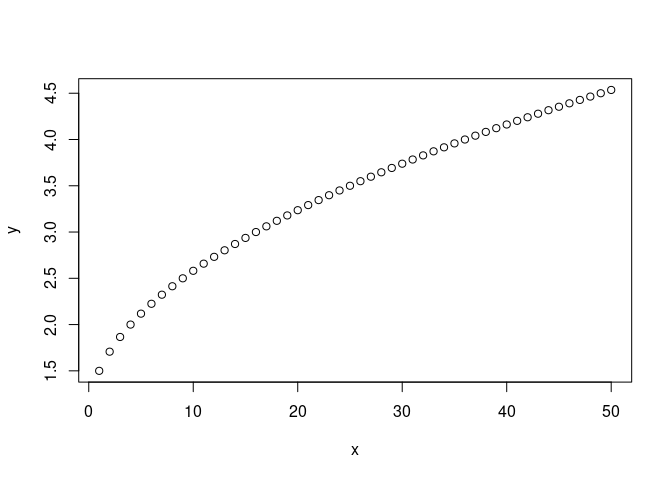
\includegraphics{embed_day3_files/figure-latex/unnamed-chunk-18-1.pdf}

\begin{Shaded}
\begin{Highlighting}[]
\FunctionTok{plot}\NormalTok{(x,y, }\AttributeTok{type=}\StringTok{"l"}\NormalTok{)}
\end{Highlighting}
\end{Shaded}

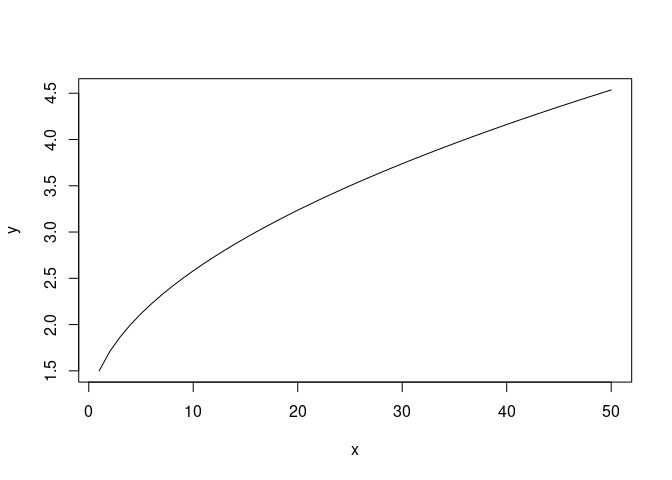
\includegraphics{embed_day3_files/figure-latex/unnamed-chunk-18-2.pdf}

\begin{Shaded}
\begin{Highlighting}[]
\CommentTok{\# plot both the points and lines}
\DocumentationTok{\#\# first plot points}
\FunctionTok{plot}\NormalTok{(x,y)}
\FunctionTok{lines}\NormalTok{(x,y, }\AttributeTok{type=}\StringTok{"l"}\NormalTok{)}
\end{Highlighting}
\end{Shaded}

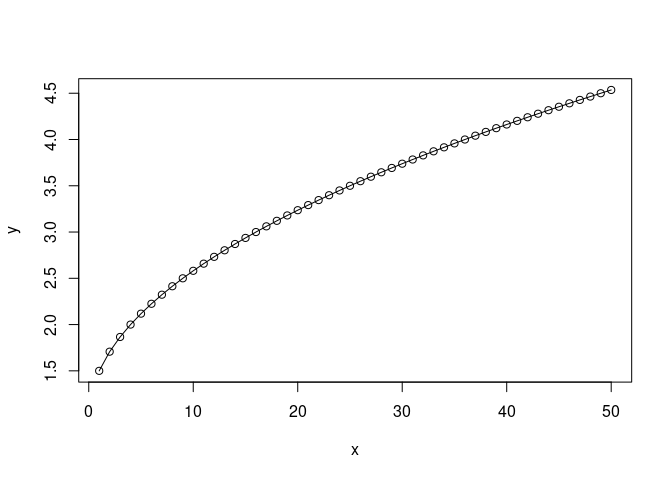
\includegraphics{embed_day3_files/figure-latex/unnamed-chunk-18-3.pdf}

\begin{Shaded}
\begin{Highlighting}[]
\DocumentationTok{\#\# lines() can only be used to add information to a graph, while it cannot produce a graph on its own.}
\end{Highlighting}
\end{Shaded}

boxplot() can be used to summarize data.

\begin{Shaded}
\begin{Highlighting}[]
\FunctionTok{boxplot}\NormalTok{(data3, }\AttributeTok{xlab=}\StringTok{"Sample ID"}\NormalTok{, }\AttributeTok{ylab=}\StringTok{"Raw Counts"}\NormalTok{)}
\end{Highlighting}
\end{Shaded}

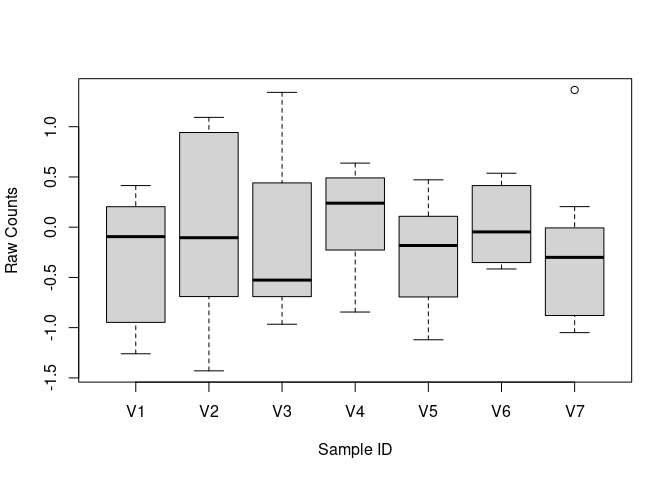
\includegraphics{embed_day3_files/figure-latex/unnamed-chunk-19-1.pdf}

\begin{Shaded}
\begin{Highlighting}[]
\NormalTok{x }\OtherTok{\textless{}{-}} \FunctionTok{rnorm}\NormalTok{(}\DecValTok{1000}\NormalTok{)}
\FunctionTok{boxplot}\NormalTok{(x)}
\end{Highlighting}
\end{Shaded}

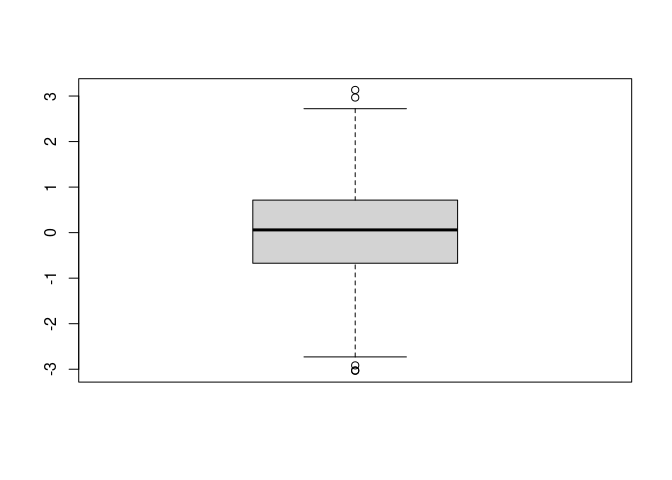
\includegraphics{embed_day3_files/figure-latex/unnamed-chunk-20-1.pdf}

hist() can be used to create histograms of data.

\begin{Shaded}
\begin{Highlighting}[]
\FunctionTok{hist}\NormalTok{(x)}
\end{Highlighting}
\end{Shaded}

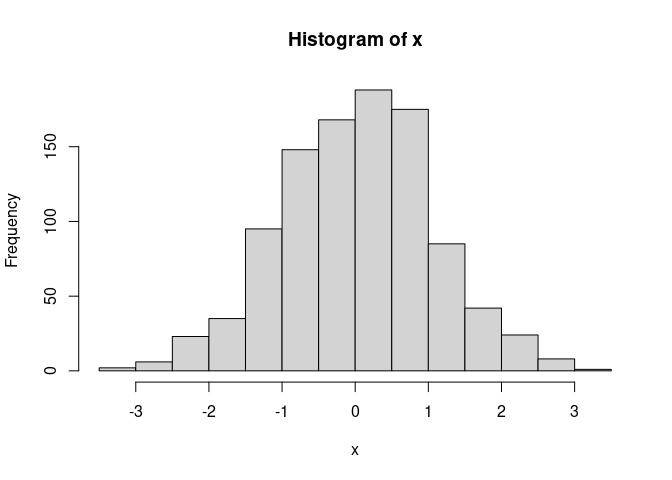
\includegraphics{embed_day3_files/figure-latex/unnamed-chunk-21-1.pdf}

\begin{Shaded}
\begin{Highlighting}[]
\CommentTok{\# use user defined break points}
\FunctionTok{hist}\NormalTok{(x, }\AttributeTok{breaks=}\FunctionTok{seq}\NormalTok{(}\FunctionTok{range}\NormalTok{(x)[}\DecValTok{1}\NormalTok{]}\SpecialCharTok{{-}}\DecValTok{1}\NormalTok{, }\FunctionTok{range}\NormalTok{(x)[}\DecValTok{2}\NormalTok{]}\SpecialCharTok{+}\DecValTok{1}\NormalTok{, }\AttributeTok{by=}\FloatTok{0.5}\NormalTok{))}
\end{Highlighting}
\end{Shaded}

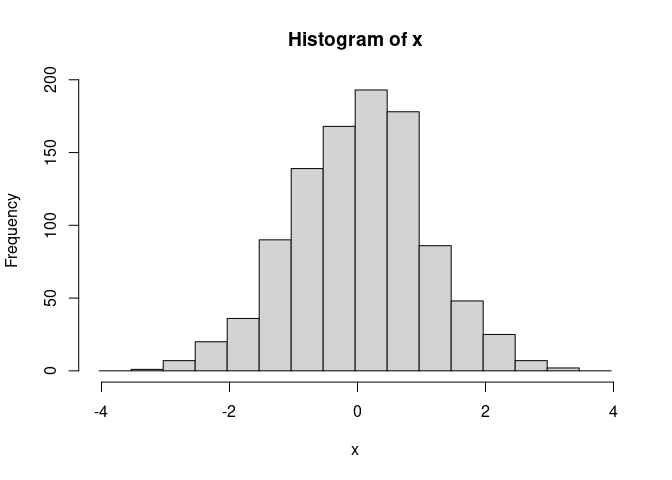
\includegraphics{embed_day3_files/figure-latex/unnamed-chunk-21-2.pdf}

\begin{Shaded}
\begin{Highlighting}[]
\CommentTok{\# clear plotting device/area}
\FunctionTok{dev.off}\NormalTok{()}
\end{Highlighting}
\end{Shaded}

\begin{verbatim}
## null device 
##           1
\end{verbatim}

\begin{center}\rule{0.5\linewidth}{0.5pt}\end{center}

\hypertarget{topic-8.-install-packages-in-r}{%
\section{Topic 8. Install packages in
R}\label{topic-8.-install-packages-in-r}}

\hypertarget{starting-from-bioconductor-version-3.8-the-installation-of-packages-is-recommended-to-use-biocmanager.}{%
\subparagraph{Starting from Bioconductor version 3.8, the installation
of packages is recommended to use
BiocManager.}\label{starting-from-bioconductor-version-3.8-the-installation-of-packages-is-recommended-to-use-biocmanager.}}

\begin{Shaded}
\begin{Highlighting}[]
\ControlFlowTok{if}\NormalTok{ (}\SpecialCharTok{!}\FunctionTok{requireNamespace}\NormalTok{(}\StringTok{"BiocManager"}\NormalTok{))}
    \FunctionTok{install.packages}\NormalTok{(}\StringTok{"BiocManager"}\NormalTok{)}
\DocumentationTok{\#\# install core packages}
\NormalTok{BiocManager}\SpecialCharTok{::}\FunctionTok{install}\NormalTok{()}
\DocumentationTok{\#\# install specific packages}
\NormalTok{BiocManager}\SpecialCharTok{::}\FunctionTok{install}\NormalTok{(}\FunctionTok{c}\NormalTok{(}\StringTok{"devtools"}\NormalTok{, }\StringTok{"tidyverse"}\NormalTok{,}\StringTok{"bsseq"}\NormalTok{,}\StringTok{"DSS"}\NormalTok{))}
\end{Highlighting}
\end{Shaded}

\begin{itemize}
\item
  Bioconductor has a repository and release schedule that differ from R
  (Bioconductor has a `devel' branch to which new packages and updates
  are introduced, and a stable `release' branch emitted once every 6
  months to which bug fixes but not new features are introduced). This
  mismatch causes that the version detected by install.packages() is
  sometimes not the most recent `release'.
\item
  A consequence of the distinct `devel' branch is that
  install.packages() sometimes points only to the `release' repository,
  while users might want to have access to the leading-edge features in
  the develop version.
\item
  An indirect consequence of Bioconductor's structured release is that
  packages generally have more extensive dependences with one another.
\end{itemize}

\hypertarget{section}{%
\subparagraph{\texorpdfstring{\textcolor{orange}{It is always recommended to update to the most current version of R and Bioconductor. If it is not possible and R < 3.5.0, please use the legacy approach to install Bioconductor packages}}{}}\label{section}}

\begin{Shaded}
\begin{Highlighting}[]
\FunctionTok{source}\NormalTok{(}\StringTok{"http://bioconductor.org/biocLite.R"}\NormalTok{)}
\DocumentationTok{\#\# install core packages}
\FunctionTok{biocLite}\NormalTok{()}
\DocumentationTok{\#\# install specific packages}
\FunctionTok{biocLite}\NormalTok{(}\FunctionTok{c}\NormalTok{(}\StringTok{"devtools"}\NormalTok{, }\StringTok{"tidyverse"}\NormalTok{,}\StringTok{"bsseq"}\NormalTok{,}\StringTok{"DSS"}\NormalTok{))}
\end{Highlighting}
\end{Shaded}

\hypertarget{the-r-function-install.packages-can-be-used-to-install-packages-that-are-not-part-of-bioconductor.}{%
\subparagraph{The R function install.packages() can be used to install
packages that are not part of
Bioconductor.}\label{the-r-function-install.packages-can-be-used-to-install-packages-that-are-not-part-of-bioconductor.}}

\begin{Shaded}
\begin{Highlighting}[]
\FunctionTok{install.packages}\NormalTok{(}\StringTok{"ggplot2"}\NormalTok{, }\AttributeTok{repos=}\StringTok{"http://cran.us.r{-}project.org"}\NormalTok{)}
\FunctionTok{install.packages}\NormalTok{(}\FunctionTok{c}\NormalTok{(}\StringTok{"kableExtra"}\NormalTok{,}\StringTok{"knitr"}\NormalTok{,}\StringTok{"dplyr"}\NormalTok{))}
\end{Highlighting}
\end{Shaded}

\hypertarget{install-from-source-of-github.}{%
\subparagraph{Install from source of
github.}\label{install-from-source-of-github.}}

\begin{Shaded}
\begin{Highlighting}[]
\FunctionTok{library}\NormalTok{(devtools)}
\FunctionTok{install\_github}\NormalTok{(}\StringTok{"stephenturner/qqman"}\NormalTok{)}
\end{Highlighting}
\end{Shaded}

\begin{center}\rule{0.5\linewidth}{0.5pt}\end{center}

\hypertarget{topic-9.-save-data-in-r-session}{%
\section{Topic 9. Save data in R
session}\label{topic-9.-save-data-in-r-session}}

\hypertarget{to-save-history-in-r-session}{%
\paragraph{To save history in R
session}\label{to-save-history-in-r-session}}

\begin{Shaded}
\begin{Highlighting}[]
\CommentTok{\#savehistory(file="Oct08.history")}

\CommentTok{\#loadhistory(file="Oct08.history")}
\end{Highlighting}
\end{Shaded}

\hypertarget{to-save-objects-in-r-session}{%
\paragraph{To save objects in R
session}\label{to-save-objects-in-r-session}}

\begin{Shaded}
\begin{Highlighting}[]
\FunctionTok{save}\NormalTok{(}\AttributeTok{list=}\FunctionTok{c}\NormalTok{(}\StringTok{"x"}\NormalTok{, }\StringTok{"data"}\NormalTok{), }\AttributeTok{file=}\StringTok{"Oct08.RData"}\NormalTok{)}

\CommentTok{\#load("Oct08.RData")}
\end{Highlighting}
\end{Shaded}

\begin{center}\rule{0.5\linewidth}{0.5pt}\end{center}

\hypertarget{topic-10.-slightly-more-advanced-visualization}{%
\section{Topic 10. Slightly more advanced
visualization}\label{topic-10.-slightly-more-advanced-visualization}}

Working with an R notebook, we will load the Iris data as we did earlier
in this documentation, generate a table that lists the median of each
measurement (Sepal.Length, Sepal.Width, Petal.Length, Petal.Width) for
each species. Then we will generate plots based on the result. Finally
produce an html report with the table and the plot.

\hypertarget{install-some-packages}{%
\paragraph{Install some packages}\label{install-some-packages}}

\begin{itemize}
\item
  In order to output a nice looking table in the final report, one may
  consider the R package kableExtra
  \url{https://github.com/haozhu233/kableExtra}. One may also check out
  the documentation at
  \url{https://cran.r-project.org/web/packages/htmlTable/vignettes/}
\item
  Figure 1 can be produced using base R functions: plot(), points(),
  axis(), text().
\item
  Figure 2 can be produced using functions in R package lattice
  \url{https://cran.r-project.org/web/packages/lattice/index.html}
\item
  Figure 3 can be produced using function boxplot()
\end{itemize}

\begin{Shaded}
\begin{Highlighting}[]
\FunctionTok{library}\NormalTok{(lattice)}
\FunctionTok{library}\NormalTok{(reshape2)}
\FunctionTok{library}\NormalTok{(kableExtra)}
\NormalTok{tmp }\OtherTok{\textless{}{-}} \FunctionTok{sapply}\NormalTok{(}\DecValTok{1}\SpecialCharTok{:}\DecValTok{4}\NormalTok{, }\ControlFlowTok{function}\NormalTok{(x)\{}\FunctionTok{tapply}\NormalTok{(iris[,x], iris[[}\DecValTok{5}\NormalTok{]], median)\})}
\FunctionTok{colnames}\NormalTok{(tmp) }\OtherTok{\textless{}{-}} \FunctionTok{colnames}\NormalTok{(iris)[}\DecValTok{1}\SpecialCharTok{:}\DecValTok{4}\NormalTok{]}
\NormalTok{nms }\OtherTok{\textless{}{-}} \FunctionTok{colnames}\NormalTok{(tmp)}
\FunctionTok{kable}\NormalTok{(}\FunctionTok{data.frame}\NormalTok{(tmp, }\AttributeTok{stringsAsFactors=}\NormalTok{F), }\AttributeTok{align=}\StringTok{\textquotesingle{}c\textquotesingle{}}\NormalTok{) }\SpecialCharTok{\%\textgreater{}\%} \FunctionTok{kable\_styling}\NormalTok{(}\AttributeTok{bootstrap\_options=}\FunctionTok{c}\NormalTok{(}\StringTok{"striped"}\NormalTok{, }\StringTok{"hover"}\NormalTok{, }\StringTok{"responsive"}\NormalTok{), }\AttributeTok{full\_width=}\NormalTok{F, }\AttributeTok{position=}\StringTok{"center"}\NormalTok{)}
\end{Highlighting}
\end{Shaded}

\begin{table}
\centering
\begin{tabular}{l|c|c|c|c}
\hline
  & Sepal.Length & Sepal.Width & Petal.Length & Petal.Width\\
\hline
setosa & 5.0 & 3.4 & 1.50 & 0.2\\
\hline
versicolor & 5.9 & 2.8 & 4.35 & 1.3\\
\hline
virginica & 6.5 & 3.0 & 5.55 & 2.0\\
\hline
\end{tabular}
\end{table}

\hypertarget{scatter-plot-of-mean-measurement}{%
\section{scatter plot of mean
measurement}\label{scatter-plot-of-mean-measurement}}

\begin{Shaded}
\begin{Highlighting}[]
\NormalTok{species }\OtherTok{\textless{}{-}} \FunctionTok{as.vector}\NormalTok{(}\FunctionTok{levels}\NormalTok{(iris}\SpecialCharTok{$}\NormalTok{Species))}
\NormalTok{x }\OtherTok{\textless{}{-}} \FunctionTok{c}\NormalTok{(}\DecValTok{1}\NormalTok{, }\DecValTok{2}\NormalTok{, }\DecValTok{3}\NormalTok{, }\DecValTok{4}\NormalTok{)}
\FunctionTok{plot}\NormalTok{(x, tmp[}\StringTok{"setosa"}\NormalTok{,], }\AttributeTok{pch=}\DecValTok{20}\NormalTok{, }\AttributeTok{col=}\StringTok{\textquotesingle{}red\textquotesingle{}}\NormalTok{, }\AttributeTok{ylim=}\FunctionTok{c}\NormalTok{(}\DecValTok{0}\NormalTok{, }\FunctionTok{max}\NormalTok{(tmp)), }\AttributeTok{xaxt=}\StringTok{"n"}\NormalTok{, }\AttributeTok{xlab=}\StringTok{"Measurement type"}\NormalTok{, }\AttributeTok{ylab=}\StringTok{"Measurement results"}\NormalTok{, }\AttributeTok{cex.lab=}\FloatTok{1.0}\NormalTok{)}
\FunctionTok{points}\NormalTok{(x, tmp[}\StringTok{"virginica"}\NormalTok{,], }\AttributeTok{pch=}\DecValTok{20}\NormalTok{, }\AttributeTok{col=}\StringTok{\textquotesingle{}orange\textquotesingle{}}\NormalTok{)}
\FunctionTok{points}\NormalTok{(x, tmp[}\StringTok{"versicolor"}\NormalTok{,], }\AttributeTok{pch=}\DecValTok{20}\NormalTok{, }\AttributeTok{col=}\StringTok{\textquotesingle{}blue\textquotesingle{}}\NormalTok{)}
\FunctionTok{axis}\NormalTok{(}\DecValTok{1}\NormalTok{, }\AttributeTok{at=}\NormalTok{x, }\AttributeTok{labels=}\NormalTok{nms, }\AttributeTok{las=}\DecValTok{2}\NormalTok{, }\AttributeTok{cex.axis=}\FloatTok{0.7}\NormalTok{)}
\FunctionTok{text}\NormalTok{(}\FunctionTok{c}\NormalTok{(}\FloatTok{1.5}\NormalTok{,}\FloatTok{1.5}\NormalTok{,}\FloatTok{1.5}\NormalTok{), }\FunctionTok{c}\NormalTok{(}\DecValTok{0}\NormalTok{, }\FloatTok{0.7}\NormalTok{, }\FloatTok{1.4}\NormalTok{), }\AttributeTok{labels=}\NormalTok{species, }\AttributeTok{col=}\FunctionTok{c}\NormalTok{(}\StringTok{"red"}\NormalTok{, }\StringTok{"blue"}\NormalTok{, }\StringTok{"orange"}\NormalTok{), }\AttributeTok{cex=}\FloatTok{1.5}\NormalTok{)}
\end{Highlighting}
\end{Shaded}

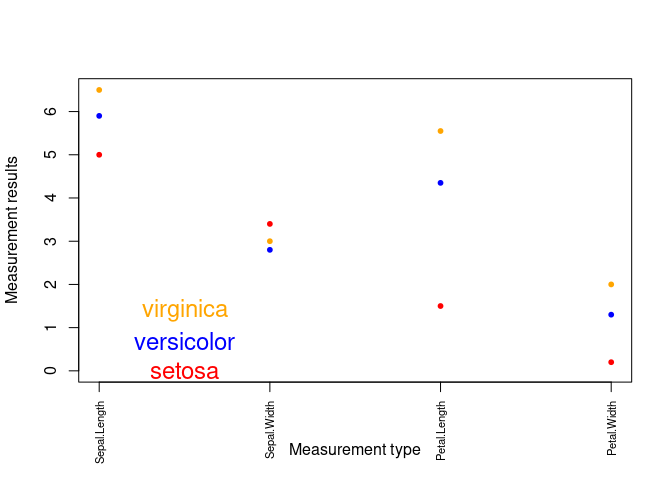
\includegraphics{embed_day3_files/figure-latex/unnamed-chunk-30-1.pdf}

\hypertarget{scatter-plot-of-measurement-by-species}{%
\section{scatter plot of measurement by
species}\label{scatter-plot-of-measurement-by-species}}

\begin{Shaded}
\begin{Highlighting}[]
\NormalTok{dd }\OtherTok{\textless{}{-}} \FunctionTok{melt}\NormalTok{(iris)}
\end{Highlighting}
\end{Shaded}

\begin{verbatim}
## Using Species as id variables
\end{verbatim}

\begin{Shaded}
\begin{Highlighting}[]
\FunctionTok{xyplot}\NormalTok{(value }\SpecialCharTok{\textasciitilde{}}\NormalTok{ variable }\SpecialCharTok{|}\NormalTok{ Species, }\AttributeTok{data=}\NormalTok{dd, }\AttributeTok{scales=}\FunctionTok{list}\NormalTok{(}\AttributeTok{x=}\FunctionTok{list}\NormalTok{(}\AttributeTok{rot=}\DecValTok{90}\NormalTok{)), }\AttributeTok{xlab=}\StringTok{"Measurements"}\NormalTok{, }\AttributeTok{ylab=}\StringTok{"Values"}\NormalTok{)}
\end{Highlighting}
\end{Shaded}

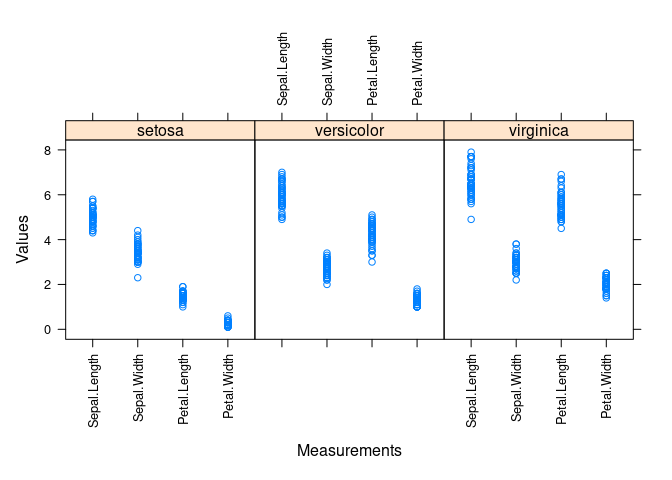
\includegraphics{embed_day3_files/figure-latex/unnamed-chunk-31-1.pdf}

\hypertarget{boxplot-by-group}{%
\section{boxplot by group}\label{boxplot-by-group}}

\begin{Shaded}
\begin{Highlighting}[]
\NormalTok{cols }\OtherTok{\textless{}{-}} \FunctionTok{c}\NormalTok{(}\StringTok{"red"}\NormalTok{, }\StringTok{"blue"}\NormalTok{, }\StringTok{"orange"}\NormalTok{)}
\FunctionTok{boxplot}\NormalTok{(value }\SpecialCharTok{\textasciitilde{}}\NormalTok{ Species }\SpecialCharTok{+}\NormalTok{ variable, }\AttributeTok{data=}\NormalTok{dd, }\AttributeTok{col =}\NormalTok{ cols, }\AttributeTok{xaxt=}\StringTok{"n"}\NormalTok{, }\AttributeTok{yaxt=}\StringTok{"n"}\NormalTok{, }\AttributeTok{xlab=}\StringTok{"Measurement Type"}\NormalTok{, }\AttributeTok{ylab=}\StringTok{"Values"}\NormalTok{)}
\FunctionTok{axis}\NormalTok{(}\AttributeTok{side=}\DecValTok{1}\NormalTok{, }\AttributeTok{labels=}\ConstantTok{FALSE}\NormalTok{)}
\FunctionTok{axis}\NormalTok{(}\AttributeTok{side=}\DecValTok{2}\NormalTok{, }\AttributeTok{las=}\DecValTok{2}\NormalTok{)}
\FunctionTok{text}\NormalTok{(}\AttributeTok{x=}\DecValTok{1}\SpecialCharTok{:}\DecValTok{12}\NormalTok{, }\AttributeTok{y=}\FunctionTok{par}\NormalTok{(}\StringTok{"usr"}\NormalTok{)[}\DecValTok{3}\NormalTok{] }\SpecialCharTok{{-}} \FloatTok{0.85}\NormalTok{, }\AttributeTok{labels=}\FunctionTok{c}\NormalTok{(}\StringTok{""}\NormalTok{, }\StringTok{"Sepal.Length"}\NormalTok{, }\StringTok{""}\NormalTok{, }\StringTok{""}\NormalTok{, }\StringTok{"Sepal.Width"}\NormalTok{, }\StringTok{""}\NormalTok{, }\StringTok{""}\NormalTok{, }\StringTok{"Petal.Length"}\NormalTok{, }\StringTok{""}\NormalTok{, }\StringTok{""}\NormalTok{, }\StringTok{"Petal.Width"}\NormalTok{, }\StringTok{""}\NormalTok{), }\AttributeTok{xpd=}\ConstantTok{NA}\NormalTok{, }\AttributeTok{srt=}\DecValTok{35}\NormalTok{, }\AttributeTok{cex=}\DecValTok{1}\NormalTok{)}
\FunctionTok{legend}\NormalTok{(}\StringTok{"topright"}\NormalTok{, }\AttributeTok{fill=}\NormalTok{cols, }\AttributeTok{legend=}\FunctionTok{levels}\NormalTok{(dd}\SpecialCharTok{$}\NormalTok{Species))}
\end{Highlighting}
\end{Shaded}

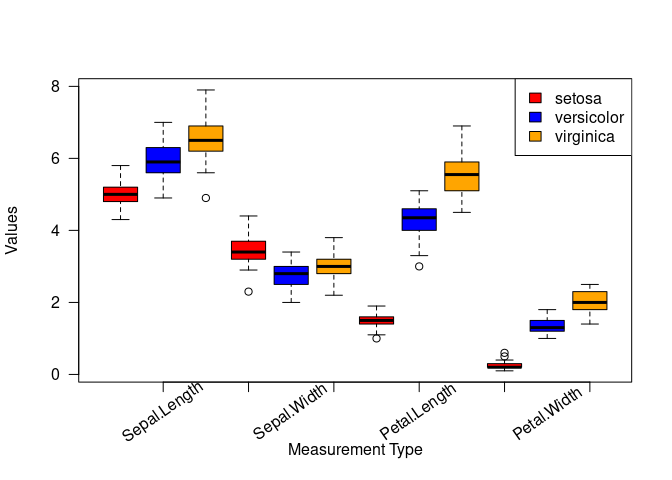
\includegraphics{embed_day3_files/figure-latex/unnamed-chunk-32-1.pdf}

\end{document}
